% !TEX root = ../../presentation.tex
% Meta: Module

\begin{slide}{Module}
  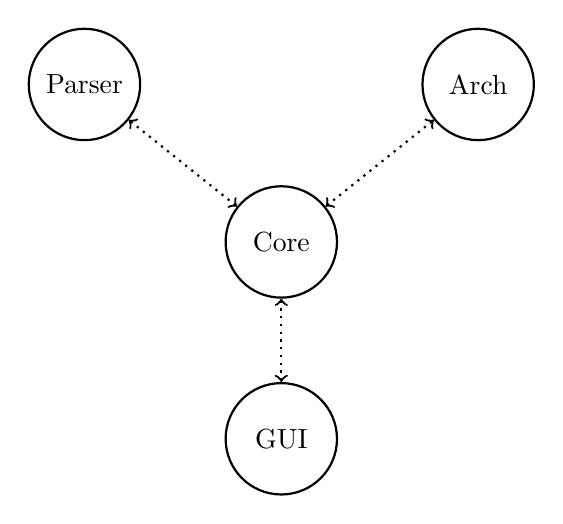
\begin{tikzpicture}[thick]
    \tikzset{module/.style={draw, circle, inner sep=0.5cm}};

    % Modules
    \onslide<5->{\path ( 0.0,  0.0) coordinate [module] (core) node {Core};}
    \onslide<2->{\path (+2.5, +2.0) coordinate [module] (arch) node {Arch};}
    \onslide<3->{\path (-2.5, +2.0) coordinate [module] (parser) node {Parser};}
    \onslide<4->{\path ( 0.0, -2.5) coordinate [module] (gui) node {GUI};}

    % Edges
    \onslide<6->{
      \draw [<->, dotted] (core) -- (arch);
      \draw [<->, dotted] (core) -- (parser);
      \draw [<->, dotted] (core) -- (gui);
    }
  \end{tikzpicture}
\end{slide}
